\subsection{Binäre Relate als Netzwerke}
\subsubsection{Definition}
Ein \emph{binäres Relat} ist erklärt als Paar $M:=(M,R)$, wobei M und R Mengen sind und
$ {R} \subseteq {M \times M }$, d.h. R ist ``binäre Relation auf M''.
\\Sei $GM := (M,R,\sigma,\tau)$ mit $\sigma : E \rightarrow V, (p,q) \mapsto p$ und $\tau : E \rightarrow V, (p,q) \mapsto q$
\\GM heiße das zu M gehörige Netzwerk bzw.  ``M=(M,R) als Netzwerke''

\begin{figure}
 \centering
 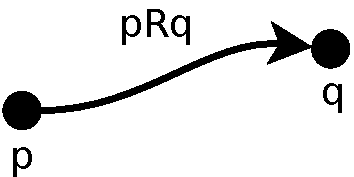
\includegraphics[scale=0.7]{../bilder/binaere_relation.pdf}
 \caption{Die Notatoin $pRq$ steht für $(p,q) \in R$, vergleiche auch Vorlesung Mathematik I, Definition 3.1.1 }
 % binäre_relation.pdf: 170x85 pixel, 72dpi, 6.00x3.00 cm, bb=0 0 170 85
\end{figure}


\paragraph{Bemerkung}
Der Begriff ``binäres Relat'' ist in der Literatur nicht verbreitet, aber für die Vorlesung zweckmäßig.